\chapter{Introduction}
\label{ch:Intro}
\par
The unifying theme in this thesis is the presence of hidden hyperbolic geometries in strongly interacting systems and their bilayers. 

What is a fermi liquid? and what is a non-fermi liquid 

Consider a scattering diagram: self energy proportional to DoS, van hove points can break fermi liquid theory. cite polchinski, shankar.

\newpage     

\section{Fermions, fermi surfaces and quasiparticles}

Condensed matter physics concerns the study of the quantum properties of matter. We know of solids to be composed of atoms arranged in a crystalline structure. Their quantum description at its core is given by the many-body Schrodinger equation of all the electrons and ions that make up the solid, all interacting with each other. The first simplification one can make is to observe that the ions in a solid are composed of a many protons and neutrons, and are much heavier than the electrons since $\nicefrac{m_p}{m_e} \approx 2000$. Then the solid's low energy dynamics can be modeled by the motion of free electrons and their interactions with each other through the electromagnetic force, and with the vibrations of the lattice, known as phonons~\cite{oppenheimer1927quantentheorie}. 

\par 
Schematically, in the language of second quantization, the hamiltonian of the system can be written as 
\begin{align}
    H \sim \underbrace{\sum_k \epsilon_k c^\dagger_k c^{\phantom{\dagger}}_k}_{T} + \underbrace{\frac{g}{\Omega}\sum_{k,k^\prime,q} c^\dagger_{k+\frac{q}{2}}c^\dagger_{k^\prime -\frac{q}{2}}c^{\phantom{\dagger}}_k c^{\phantom{\dagger}}_{k^\prime}}_{V} \quad\quad, 
    \label{eq:schemHam}
\end{align}
where the kinetic and potential energy terms have been separated out. In Eq.~\eqref{eq:schemHam}, $\epsilon_k$ refers to the dispersion of bare electrons subject to the symmetry of the lattice, and $\Omega$ is the volume of the system under consideration. For simplicity, all interactions that the electrons are subject to are schematically represented by the constant $g$, which may come from their charged interactions or with phonons or impurities etc. In a real material, the interaction itself may have a long range (and hence a momentum dependance), or may even face retardation effects, but these are neglected for now. 

\par
Let's first consider the kinetic energy term, given by $T$, and let us also suppose the bare parabolic dispersion of free electrons in the Galilean continuum: 
\textbf{INSERT FIGURE OF PARABOLA GETTING FILLED WITH STATES TILL FERMI ENERGY}
Just the fact that electrons are fermions obeying the Pauli exclusion principle means that the large density of free electrons in a metal corresponds to a gigantic energy scale. For example, in copper~\cite{Ashcroft1976} which has an electron density of $8.47\times 10^{28} m^{-3}$, the energy of the topmost occupied level turns out to be $7 eV$, which corresponds to about $81600 K$ in units of temperature. For reference, the surface of the sun is at a temperature of $5000 K$. 
\par 
This mammoth fermi energy is what is responsible in most cases to the success of Landau's fermi liquid theory. To lowest approximation, electrons can be considered to be completely non-interacting, from which weak interactions can be included perturbatively~\cite{luttinger1960ground,baym1961conservation,pines2018microscopic}. 
\par 
This can be understood mathematically using the language of Green's functions. The Dyson equation can be written as 
\begin{equation}
    G(\vec{k},\omega) = \frac{1}{\omega - \epsilon_{\vec{k}} - \Sigma(\vec{k},\omega)}
\end{equation}
 Typically, the green's function for free fermions looks like \begin{equation}
        G^0(k,\omega) = \frac{1}{\omega - \xi_k}
    \end{equation}
 The characteristic feature is that the green's function has poles in it. When interactions are included, the green's functions pick up a self energy according to the Dyson's equation:
 \begin{equation}
         G^{-1} = G_0^{-1} - \Sigma
 \end{equation}

The self-energy will have a frequency and momentum dependence, and also a real and an imaginary part. We can expand the self-energy around a vector on the fermi surface, at low frequencies
\begin{equation}
    \Sigma(k,\omega) = const + k\pdv{\Sigma(k,0)}{k}\eval_{k=k_F} + \omega\pdv{\Sigma(k_F,\omega)}{\omega}\eval_{\omega=0} + \cdots
\end{equation}
We can use this to rewrite the Green's function in the well-known form
\begin{align}
    G(k,\omega) &= \frac{1}{\omega\left(1 - \pdv{\Sigma}{\omega} \right) - \left(\xi_k + k\pdv{\Sigma}{k}\right) + i\Gamma} \nonumber \\ 
    &= \frac{Z}{\omega - \Tilde{\xi_k} + i\Tilde{\Gamma}} 
\end{align}
The quasiparticle residue is given by 
\begin{equation}
    Z = \left(1-\pdv{\Sigma(k_F,\omega)}{\omega}\eval_{\omega=0}\right)^{-1}
\end{equation}
Typically, if the self energy is analytic ($\Sigma \sim \alpha + \beta\omega + \gamma\omega^2 + \cdots$), the quasi-particle residue would be finite
When the derivative of the self energy blows up in the infrared(as $\omega\xrightarrow{}0$), it leads to a breakdown of fermi liquid theory. 
\par
At this point, one can mention a proposal from the past~\cite{varma1989phenomenology,ruckenstein1991theory,varma1993towards,varma2002singular}. The marginal or singular fermi liquid is the most marginal way to create non-fermi liquid behavior 
The real part of the self energy goes as 
\begin{equation}
    \Sigma \sim \omega\log(\frac{\omega}{\omega_c})
\end{equation}
\begin{figure}
    \centering
    \begin{subfigure}[b]{0.4\textwidth}
    \centering
    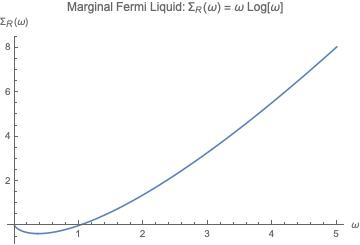
\includegraphics[width = \textwidth]{figures/introduction/MFLS.jpeg}
    \end{subfigure}
    \begin{subfigure}[b]{0.4\textwidth}
    \centering
    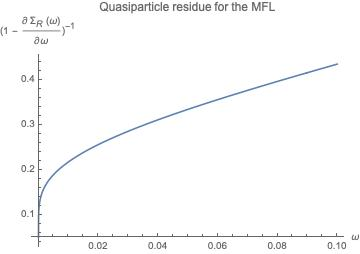
\includegraphics[width = \textwidth]{figures/introduction/MFLZ.jpeg}
    \end{subfigure}
    \caption{Absence of Quasiparticles in the marginal fermi liquid}
    \label{fig:MFLZ}
\end{figure}

\par
 We can understand the emergence of non-fermi liquid behavior as a non-analytic behavior in the self energy. 
The Green's function would now not have poles, but rather branch cuts on the $\omega$ axis. 
\par
We would like some microscopic model which helps us understand such a singular self energy.
Such an example is the SYK model, whose self energy, as we shall see goes as $\left|\omega\right|^{\nicefrac{1}{2}}$. 
\begin{figure}
    \centering
    \begin{subfigure}[b]{0.4\textwidth}
    \centering
    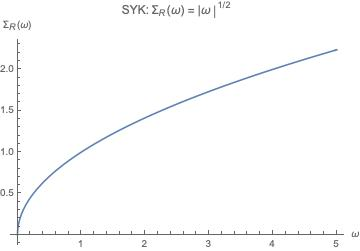
\includegraphics[width = \textwidth]{figures/introduction/SYKS.jpeg}
    \end{subfigure}
    \begin{subfigure}[b]{0.4\textwidth}
    \centering
    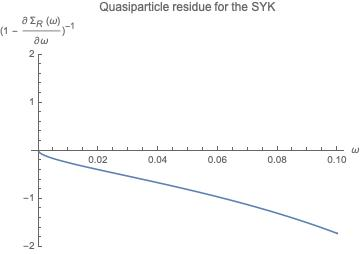
\includegraphics[width = \textwidth]{figures/introduction/SYKZ.jpeg}
    \end{subfigure}
    \caption{Absence of Quasiparticles in the SYK model}
    \label{fig:SYKZ}
\end{figure}

\section{The SYK model}
The SYK model describes the physics of interacting fermions living on a strongly disordered quantum dot. It's simplest version can be constructed using a Hamiltonian of $N$ flavors of majorana fermions interacting all-to-all with Gaussian random couplings. 
\begin{equation}
    H = \displaystyle \sum_{1\leq i<j<k<l\leq N} J_{ijkl}\,\psi_i\psi_j\psi_k\psi_l
\end{equation}
The random couplings are normally distributed, i.e 
\begin{align}
    \expval{J_{ijkl}} &= 0 \\
    \expval{J^2_{ijkl}} &= \frac{6 J^2}{N^3}
\end{align}

\par
We can look in Euclidean time. The free part of the Green's function is (with the strange normalization $\anticommutator{\psi_i}{\psi_j} = \delta_{ij}$)
\begin{align}
    G^0(\tau) &= -\expval{\mathcal{T}\psi_i(\tau)\psi_j(0)}\nonumber\\
    &= -\frac{1}{2}\sgn(\tau) \, \delta_{ij}
\end{align}
In Fourier space,  
\begin{align}
    G^0(\omega) = \int \dd\tau \,e^{i\omega\tau} G^0(\tau) = \frac{1}{i\omega}
\end{align}

\par

Upon turning on interactions, we can look at the so called melon diagrams
\begin{figure}
    \centering
    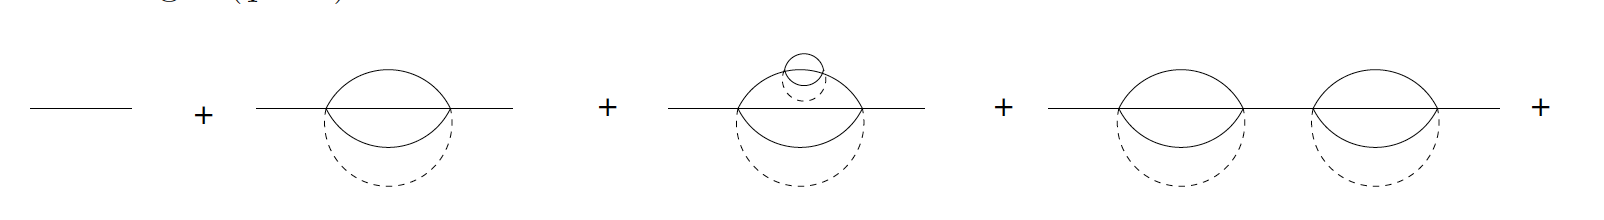
\includegraphics[width = \linewidth]{figures/introduction/SYK1.png}
    \caption{Diagrams that dress the propagator}
    \label{fig:SYK1}
\end{figure}
The disorder average means that the flavors of the four majoranas at both the connecting vertices are identical, and brings out a contribution $\sim \frac{J^2}{N^3}$ for each vertex pair. 
This combined with the large N limit forces the interacting green's function $G_{ij}(\tau) = G(\tau)\delta_{ij}$
  


\subsection{The SYK self consistent equations}
\par
With these considerations, the Dyson's equations can be represented as
\begin{figure}
    \centering
    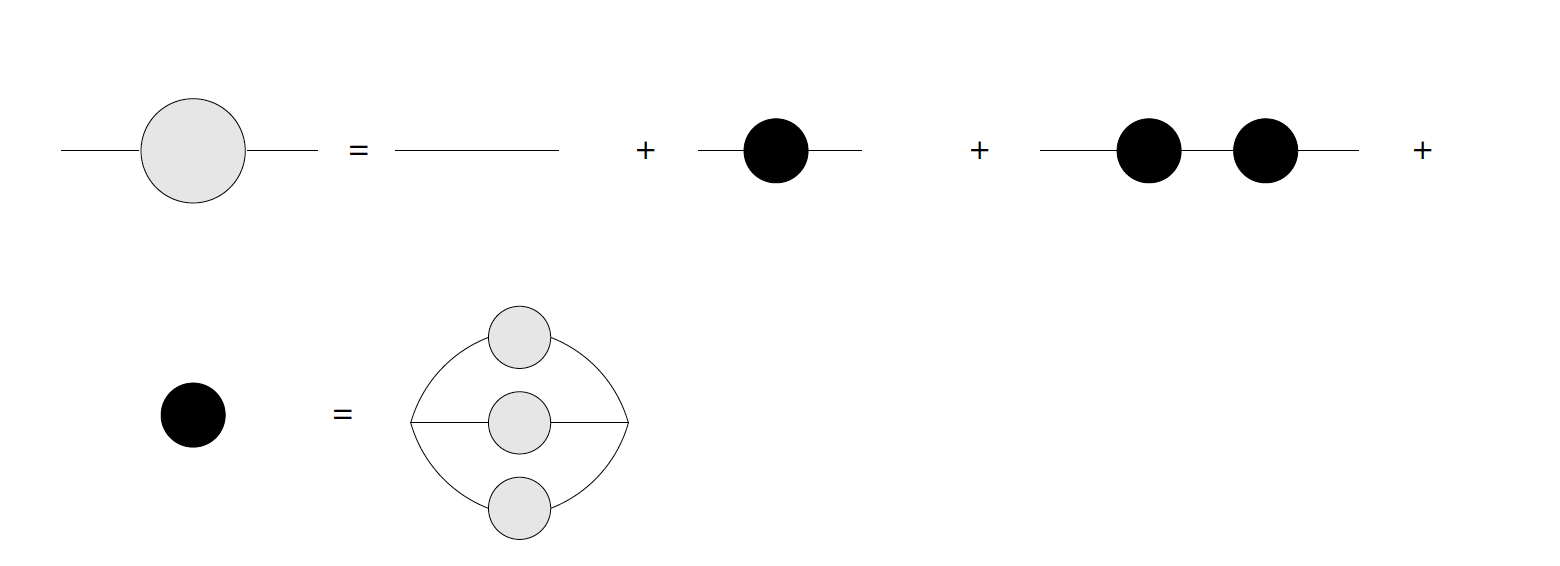
\includegraphics[width= \linewidth]{figures/introduction/Melons.png}
    \caption{Summing the Dyson series. Figure used from ~\cite{maldacena_comments_2016}}
    \label{fig:melons}
\end{figure}
  

\par
This gives us the SYK equations: 
\begin{align}
    \left(G(\omega)\right)^{-1} = i\omega - \Sigma(\omega) \label{eq:sykeq1} \\ 
    \Sigma(\tau) = J^2\left(G(\tau)\right)^3 \label{eq:sykeq2}
\end{align}
These are a set of equations that must be solved self-consistently: eq.(\ref{eq:sykeq1}) tells how the self-energy determines the Green's function, and eq.(\ref{eq:sykeq2}) says how the self-energy is set by the Green's function. 
They are not the most trivial to solve, since one is in real space, and the other in Fourier space. 
  

\par
The key to doing so is to assume that the self-energy dominates the free propagator's contribution at strong coupling in the IR $(\omega \xrightarrow{} 0)$
Then, eq.(\ref{eq:sykeq1}) can be written as:
\begin{equation}
    \int \dd\tau^\prime G(\tau,\tau^\prime)\Sigma(\tau^\prime,\tau^{\prime\prime}) = -\delta(\tau - \tau^{\prime\prime})
\end{equation}
This is solved by the ansatz
\begin{equation}
    G_c(\tau) = \frac{b\sgn(\tau)}{\abs{\tau}^{2\Delta}}
    \label{eq:Gc}
\end{equation}



\subsection{SYK as an NCFT in the IR}
\par
We see that eq.(\ref{eq:Gc}) is the form of the Green's function of a conformal field theory
$\Delta$ can be easily determined by a scaling argument $\tau \xrightarrow{} b\tau$
\begin{align}
    b^{1 - 2\Delta - 6\Delta} &= b^{-1} \nonumber \\
    \implies \Delta &= \frac{1}{4}
\end{align}
Using the identity
\begin{equation}
    \int_{-\infty}^\infty \dd\tau e^{i\omega\tau} \frac{\sgn(\tau)}{\abs{\tau}^{2\Delta}} \sim \abs{\omega}^{2\Delta-1},
\end{equation}
we retrieve our branch-cut propagator result of $\Sigma(\omega)\sim \abs{\omega}^{\nicefrac{1}{2}} $, as promised!


\section{Other versions of the SYK used in this thesis}
It would be quite a fallacy to limit one's understanding of the physics of the SYK model to simply an artificial description of majorana fermions in quantum dots. The physical content of the SYK model describes the emergence and the weak breaking of a new conformal symmetry in the infrared. Indeed, the original UV-completion of the SYK model was described by a random heisenberg coupled spin system~\cite{sachdev1993gapless}. There are also other UV-completions to include a conserved U(1) charge using complex fermions by means of the appropriately dubbed "complex-SYK"~\cite{sachdev2015bekenstein}. 
\subsection{b-SYK}
Given the importance of the SYK model, attempts have been made in order to realise it in an experimental situation. A comprehensive list of these attempts is provided in the recent review~\cite{chowdhury_sachdev-ye-kitaev_2021}. 

\par 
We will here first specifically mention Ref.~\cite{Chen2018} using graphene flakes. It is well known in graphene that the presence of a strong magnetic field induces the formation of landau levels, the lowest of which is pinned to zero energy. This completely flat band quenches the kinetic energy in Eq.~\ref{eq:schemHam}. The wavefunctions have non-trivial quantum geometry still and instead of being localized, are extended throughout the surface of the graphene. There is a zero mode generated for every quantum of flux that penetrates the sample, as is well known from the theory of the quantum hall effect. 

\par
The effects of the coulomb interaction projected onto the degenerate states of the flat band, next nearest neighbor hoppings and random onsite disorder all contribute to make the effective interactions seem almost completely random. 

\par
To provide evidence that the Hamiltonian thus generated is SYK like, the authors of  Ref.~\cite{Chen2018} took recourse to random matrix theory. They first calculated the coupling constants of the projected graphene hamiltonian by explicit numerical diagonalization as a function of flux. They observed with increasing flux that as a new zero mode was added, the distribution of couplings changed random matrix universality class, in close analogy to the Altland-Zirnbauer classification for non-interacting hamiltonians~\cite{altland1997nonstandard,fidkowski2010effects,fidkowski2011topological}, and this matches perfectly with the random matrix classes as a function of the number of fermions in the SYK model~\cite{garcia2016spectral,behrends2019tenfold,you2017sachdev}. 

\par 
A similar idea was used by Fremling and Fritz~\cite{fremling_bipartite_2021} to propose an experimental realization of a majorana version of the SYK model. They consider the Kitaev honeycomb model of spins~\cite{kitaev2006anyons}, which is believed to be realized in many spin liquid candidates including the iridates like $\mathrm{Na}_2\mathrm{IrO}_3$, $\mathrm{H}_3\mathrm{Li}\mathrm{Ir}_2\mathrm{O}_6$ and more prominently in $\alpha-\mathrm{RuCl}_3$~\cite{trebst2022kitaev,banerjee2017neutron}. The low energy theory of the Kitaev honey comb model exhibits deconfinement of the spins into majorana fermions. Fremling and Fritz noted that an analogue of a strong magnetic field creating flat landau levels could be simulated by application of triaxial strain, and the remnant interactions in these materials, for instance the heisenberg interaction, projected onto these majorana zero modes resulted in an SYK-like interaction.
\par
The catch, however, is that unlike the complex fermion case in the graphene flakes, these residual interactions are only non-vanishing for pairs of majoranas on opposite sublattices of the bipartite honeycomb lattice(see Fig.\ref{fig:bsyk}). This leads to the emergence of the so-called bipartite SYK model (b-SYK), whose hamiltonian is given by 
\begin{equation}
    H_{b-SYK} = \frac{1}{4}\sum_{i,j=1}^{N_A}\sum_{\alpha,\beta = 1}^{N_B} J_{ij\alpha\beta}\psi^A_i\psi^A_j\psi^B_\alpha\psi^B_{\beta}. 
    \label{eq:Hbsyk}
\end{equation}
Again, the couplings have some sense of Gaussianity: 
\begin{equation}
    \expval{J_{ij\alpha\beta}\,J_{i^\prime j^\prime \alpha^\prime \beta^\prime}} = \frac{J^2}{2\sqrt{N_A N_B}^3}\delta_{i,i^\prime}\delta_{j,j^\prime}\delta_{\alpha,\alpha^\prime}\delta_{\beta,\beta^\prime}
\end{equation}
Here, $N_A$ and $N_B$ are the number of sites in the $A-$ and $B-$ sublattice respectively, and need not be the same in a disordered system.
\par
Although the new model in eq.~\ref{eq:Hbsyk} contains only $\nicefrac{3}{8}$ of the non-zero couplings as the full all-to-all SYK model, it still shows an emergent conformal symmetry at low energy, with a different tunable conformal dimension for the majoranas in each set~\cite{Fremling_2022}. Such generalizations of the SYK model created by repeated pruning of the fully connected graph of couplings falls into the family of the so called "sparse SYK" models~\cite{xu_sparse_2020,garcia-garcia_sparse_2021,caceres2021sparse,caceres2023out}.

\begin{figure}
    \centering
    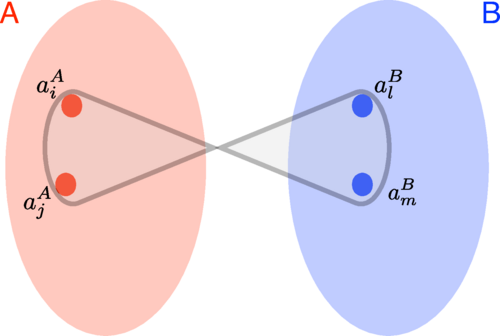
\includegraphics[scale = 0.5]{figures/introduction/bSYK.png}
    \caption{Schematic of the b-SYK model. There are 2 sets of majorana fermions living on each of the two bipartite lattices of the honeycomb lattice. The interactions of the model are such that the majoranas do not interact within a set, but every pair of majorana degrees of freedom in each set interacts with a Gaussian random coupling with every pair of majoranas on the other set. Figure from Ref.~\cite{Fremling_2022}.}
    \label{fig:bsyk}
\end{figure}

\subsection{Yukawa-SYK model}
The SYK model can also be generalized to include bosonic degrees of freedom. The Yukawa SYK (y-SYK) model can be thought of as a zero dimensional analogue of the electron-phonon coupling hamiltonian. This has been the subject of intense theoretical study in recent years~\cite{esterlis2019cooper,wang2020quantum,wang2020solvable,classen2021superconductivity,inkof2022quantum,pan2021yukawa,davis2023quantum,grunwald2024dynamical,choi2022pairing}. The model also allows for a generalization into higher dimension for a recently proposed universal theory of strange metals~\cite{patel2023universal,valentinis2023correlation,esterlis2021large,guo2022large,guo2023large,li2024strange} by being able to have a controlled large-N limit overcoming previous challenges~\cite{lee2009low}.

\par
The hamiltonian for the Yukawa SYK is very reminiscent of the Fr\"ohlich hamiltonian for the electron-phonon interaction and can be written as 
\begin{equation}
    H_{Y-SYK} = -\mu\sum_{i=1}^N\sum_\sigma c^\dagger_{i,\sigma} c^{\phantom{\dagger}}_{i, \sigma} + \sum_{k=1}^M \frac{1}{2}\left(\pi_k^2 + \omega_0^2\phi_k^2\right) + \frac{\sqrt{2}}{N}\sum_{i,j,k}\sum_{\sigma}g_{ijk} c^\dagger_{i,\sigma} c^{\phantom{\dagger}}_{j,\sigma} \phi^{\phantom{\dagger}}_k .
    \label{eq:HYSYK}
\end{equation}
The are $N$ flavors of fermions, and $M$ flavors of bosons, and we are interested in the regime when both $N\rightarrow\infty, M\rightarrow\infty, \, \kappa = \frac{M}{N}$ held constant. 

\par
In the absence of time reversal symmetry, for the hamiltonian to be hermitian, the couplings $g_{ij,k}$ have to satisfy 
\begin{equation}
    g_{ji,k} = g^*_{ij,k},
\end{equation}
and are drawn from the Gaussian unitary ensemble (GUE). At zero temperature, the low energy theory in this case is completely akin to the conventional syk non-fermi liquid, and develops an emergent conformal symmetry, with a scaling dimension set by $\kappa$. 
The Schwinger-Dyson equations in this case read
\begin{align}
    \Sigma(\tau) &= \kappa \, g^2 \, G(\tau) D(\tau) \\
    \Pi(\tau) = &= -2g^2 \, G(\tau)G(-\tau) \\
    G(i\omega_n) &= \frac{1}{i\omega_n + \mu - \Sigma(i\omega_n)} \\
    D(i\nu_n) &= \frac{1}{\nu_n^2 + \omega_0^2 - \Pi(i\nu_n)} .
    \label{eq:SchDysEqnsYSYK_Imag}
\end{align}
The model is self-tuning to criticality~\cite{esterlis2019cooper}, i.e the bosons modes soften in the infrared. This is the condition that at zero temperature, $\Pi(\omega = 0) = \omega_0^2$
In the infrared, they can be solved with the zero-temperature conformal ansatz 
\begin{align}
    G(\tau) &= b\frac{\sgn(\tau)}{\abs{\tau}^{2\Delta_f}} ,\\
    D(\tau) &= d\frac{1}{\abs{\tau}^{2\Delta_b}} .
\end{align}
These can be Fourier transformed using the identities
\begin{align}
        \int_{-\infty}^{\infty} d\tau\,\frac{\sgn(\tau)}{\abs{\tau}^\alpha} e^{i\omega\tau} &= i2^{1-\alpha}\sqrt{\pi}\frac{\Gamma(1-\frac{\alpha}{2})}{\Gamma(\frac{1}{2}+\frac{\alpha}{2})}\abs{\omega}^{\alpha-1}\sgn(\omega) , \\
        \int_{-\infty}^{\infty} d\tau\,\frac{1}{\abs{\tau}^\alpha} e^{i\omega\tau}  &= 2^{1-\alpha}\sqrt{\pi}\frac{\Gamma(\frac{1}{2}-\frac{\alpha}{2})}{\Gamma(\frac{\alpha}{2})}\abs{\omega}^{\alpha-1}. 
\end{align}
We then get 
\begin{align}
    \Sigma(\omega) &= \kappa \, g^2 bd \, i2^{1-2(\Delta_f + \Delta_b)}\sqrt{\pi}\frac{\Gamma(1-(\Delta_f+\Delta_b))}{\Gamma(\frac{1}{2} + \Delta_f + \Delta_b)} \abs{\omega}^{2(\Delta_f+\Delta_b)-1}\sgn(\omega) \\
    \Pi(\omega) &= 2g^2b^2 \, 2^{1-4\Delta_f}\sqrt{\pi} \frac{\Gamma(\frac{1}{2} - 2\Delta_f)}{\Gamma(2\Delta_f)}\abs{\omega}^{4\Delta_f-1}\\
    G(\omega) &= b\,i2^{1-2\Delta_f}\sqrt{\pi}\frac{\Gamma(1-\Delta_f)}{\Gamma(\frac{1}{2}+\Delta_f)}\abs{\omega}^{2\Delta_f-1}\sgn(\omega) \\
    D(\omega) &= d\,2^{1-2\Delta_b}\sqrt{\pi}\frac{\Gamma(\frac{1}{2}-\Delta_b)}{\Gamma(\Delta_b)} \abs{\omega}^{2\Delta_b-1}
    \label{eq:scalingsolns}
\end{align}
The Dyson equation in the fully conformal limit, where the self energy wins over the free propagators are: (for now we work with $\mu = 0$ )
\begin{align}
    G(\omega)\Sigma(\omega) = -1 = D(\omega)\Pi(\omega).
    \label{eq:DysonFreq}
\end{align}
We see that in this case, only the product $b^2d$ is fixed in this fully conformal limit, and not separately the constants $b$ and $d$ themselves, as happens for regular SYK. However, this is an artifact of neglecting the short time, high frequency terms in the Dyson equation, and including the full UV corrections enables one to fix these constants, similar to the b-SYK model. The easy way to see this is that at short time, the free part of the Dyson equation should win over, and $G(\tau = 0^+)$ should be $-\frac{1}{2}\sgn(\tau)$, which is the fourier transform of $\frac{1}{i\omega}$.   

\par
Eq.\eqref{eq:scalingsolns} and Eq.~\eqref{eq:DysonFreq} together imply that
\begin{align}
    2\Delta_f + \Delta_b &= 1 ,\\
    \kappa \, \frac{\Gamma(1-\Delta_f)\Gamma(1-(\Delta_f+\Delta_b))}{\Gamma(\frac{1}{2}+\Delta_f)\Gamma(\frac{1}{2}+\Delta_f+\Delta_b)} &= -2 \frac{\Gamma(\frac{1}{2}-\Delta_b)\Gamma(\frac{1}{2}-2\Delta_f)}{\Gamma(\Delta_b)\Gamma(2\Delta_f)}.
\end{align}
For $\kappa = 1$, these equations are solved by $\Delta_f = 0.420374$, and $\Delta_b = 0.159252$.

\par 
At finite temperature, the model exhibits a rich phase diagram first outlined in Ref.~\cite{esterlis2019cooper}. For $g<1$, the highest temperatures are characterized by a limit of free fermions, where $G(\omega_n) \rightarrow \frac{1}{i\omega_n}$, and the low temperature phase is the finite temperature version of the non-fermi liquid described above. The $g>1$ regime is characterized by a novel impurity like phase at intermediate and high temperature.

\par
In the presence of time reversal symmetry, the couplings in Eq.~\eqref{eq:HYSYK} are further constrained to be completely real, and $g_{ij,k}$ have to be drawn from the Gaussian orthongoanl ensemble (GOE)
Similar to the Fr\"ohlich or the Bardeen-Pines hamiltonian, the bosons condense in the ground state of the model causing the fermions to pair with their time reversal partners. 
\par 
In this case, the non-fermi liquid metallic phase is difficult to observe as it competes with the superconducting phase, which satisfies the quantum critical Eliashberg equations~\cite{chubukov2020interplay,abanov2020interplay}. 
















\section{Graphene and its bilayers}
\label{sec:graphene}
Graphene is a single sheet of carbon atoms arranged in a hexagonal lattice~\cite{neto2009electronic}. Its electronic properties can be described by a simple tight binding model which accounts for electrons hopping between nearest neighbors in its two sublattices, with its hamiltonian given by
\begin{align}
    H &= -t \sum_{\langle i,j\rangle} a_i^\dagger b_j + h.c ,  
\end{align}
and can be diagonalized in terms of two component wavefunctions 
\begin{align}
    \Psi_i = \mqty(a_i \\ b_i  ) .
\end{align}
to obtain a spectrum given by 
\begin{align}
    E(\Vec{k}) &= \pm \sqrt{1 + 4\cos{\left(\frac{3 k_x a}{2}\right)}\cos{\left(\frac{\sqrt{3}k_y a}{2}\right)} + 4\cos^2{\left(\frac{\sqrt{3}k_y a}{2}\right)}}
    \label{eq:Graphene dispersion}
\end{align}

\begin{figure}[]
	\centering
	\begin{subfigure}{0.5\linewidth}
		\centering
		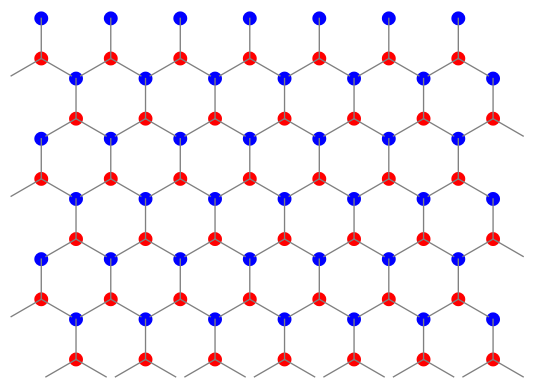
\includegraphics[width=4cm]{figures/introduction/graphene lattice.png}
            \caption{\centering}
	\end{subfigure}%
        \begin{subfigure}{0.5\linewidth}
		\centering
		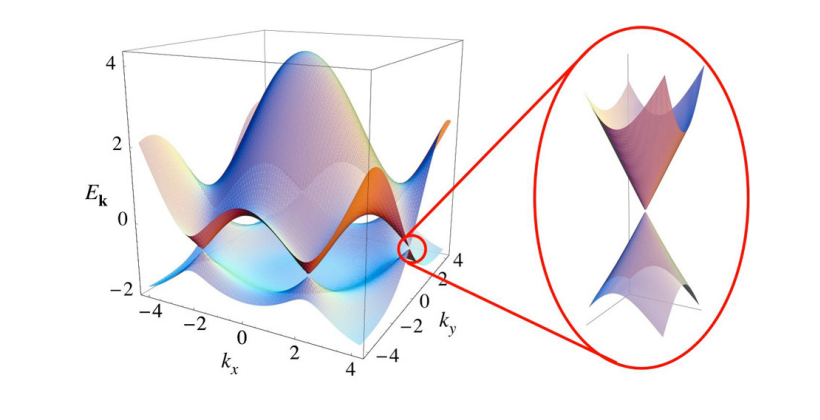
\includegraphics[width=5cm]{figures/introduction/bandstructure_graphene.png}
            \caption{\centering}
	\end{subfigure}%
	
 	\centering
	\begin{subfigure}{0.45\linewidth}
		\centering
		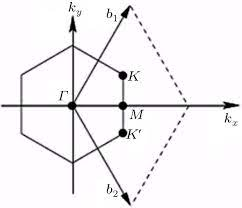
\includegraphics[width=4cm]{figures/introduction/brilluoinzonegraphene.png}
            \caption{\centering}
	\end{subfigure}
	\begin{subfigure}{0.45\linewidth}
		\centering
		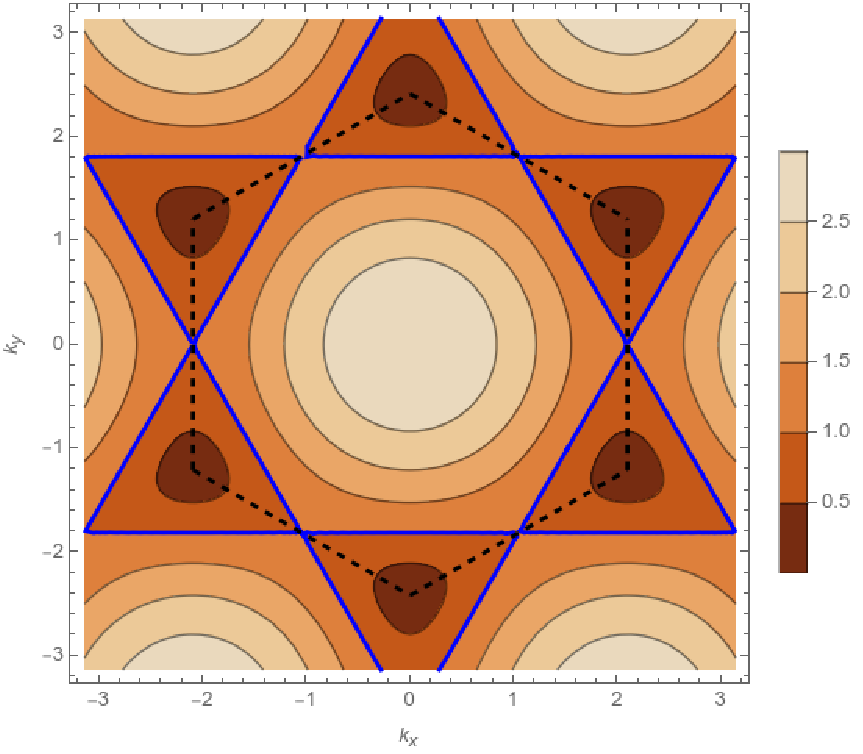
\includegraphics[width=4cm]{figures/introduction/graphenecontours.pdf}
            \caption{\centering}
	\end{subfigure}

	\caption{(a) Schematic hexagonal lattice of graphene showing carbon atoms in the A(red) and B(blue) sublattices. (b) Dispersion with zoom near the band-touching Dirac point. (c) The corresponding Brillouin zone marking the positions of the high symmetry points. (d) Energy contours of graphene showing the brilluoin zone in black dashed lines. The highlighted contour in blue is at the van Hove energy. (panels (b) and (c) taken from \cite{neto2009electronic}).}
	\label{fig:grapheneschematic}
\end{figure}

The dispersion in Eq.~\eqref{eq:Graphene dispersion} shows interesting features at the $K, K^\prime$ and the $M$ points of the Brilluoin zone. 

\par
The $K$ point and its time reversed partner $K^\prime$ points are referred to as Dirac points. This is because the gap between the two bands closes at these points, and the dispersion is linear. Indeed, the low energy hamiltonian close to for momenta $\vec{p}$ close to the $K$ point can be represented as 
\begin{align}
    H = v_F \,\Vec{p} \cdot \Vec{\sigma}.
    \label{eq:DiracHam}
\end{align}
\par 
The Dirac matrices in two dimensions are simply the $2x2$ Pauli matrices given by $\vec{\sigma}$. 
The corresponding dispersion $E(\Vec{p}) = v_F \abs{\vec{p}}$ is dubbed a Dirac cone, because it looks like a causal light cone from special relativity, just with an effective speed of light $v_F$. 

\par 
Graphene also has an interesting saddle-like dispersion near its $M$ point. This is shown in panels (b) and (d) of Fig.\ref{fig:grapheneschematic}. 
Since first derivatives vanish at a saddle point, the dispersion is most faithfully captured by a Taylor expansion upto second order, with the expansion coefficients in the two principal directions having opposite sign: 
\begin{equation}
    E = E_v + \alpha p_x^2 -\beta p_y^2 \quad\quad \alpha,\beta>0
    \label{eq:dispQUAD}
\end{equation}
Then, we can find the density of states: 
\begin{equation}
    \rho(E) = \int \frac{\dd p_y}{2\pi} \frac{\dd p_x}{2\pi} \, \delta(E - E_{\vec{p}})
    \label{eq:DOSformula}
\end{equation}
where we use the formula 
\begin{equation}
    \delta(g(x)) = \sum_i \frac{\delta(x-x_i)}{\abs{g^\prime(x_i)}}
\end{equation}
where $x_i$ are the roots of the function $g(x)$. Here we have $g(p_x) = E - E_v +\beta p_y^2 - \alpha p_x^2$, and $g^\prime(p_x) = -2\alpha p_x$. 
We obtain the roots of $g(p_x)$ as 
\begin{equation}
    p_x^\pm = \pm\sqrt{\frac{(E-E_v)+\beta p_y^2}{\alpha}}
\end{equation}
which gives, defining $\Tilde{E} = E - E_v$ 
\begin{equation}
    \rho(E) = \int \frac{\dd p_y}{2\pi} \int_{-\infty}^\infty \frac{\dd p_x}{2\pi} \, \frac{\delta(p_x - p_x^+) + \delta(p_x - p_x^-)}{2\sqrt{\alpha\beta}\sqrt{\frac{\Tilde{E}}{\beta} + p_y^2}}
\end{equation}

A note has to be made here about the range of $p_y$, which comes from the condition when $p_x$ has a solution, which is when $E - E_v + \beta p_y^2 > 0$. 

\begin{equation}
    \text{range of } p_y =
    \begin{cases} 
    \texttt{True}, \quad E>E_v \\
    p_y^2 > \abs{\frac{E-E_v}{\beta}}, \quad E<E_v
    \end{cases} 
\end{equation}

Introducing a cutoff for $p_y$ as $\Lambda$, for $E>E_v$, 
\begin{align}
    \rho(E) &= \frac{2}{\sqrt{\alpha\beta}} \int_0^\infty \frac{\dd p_y}{(2\pi)^2} \frac{1}{\sqrt{\frac{\Tilde{E}}{\beta} +  p_y^2}} \nonumber \\
    &= \frac{1}{2\pi^2\sqrt{\alpha\beta}} \log\abs{\frac{2\Lambda\sqrt{\beta}}{\sqrt{E - E_v}}} \nonumber \\
    &= \frac{1}{4\pi^2 \sqrt{\alpha\beta}} \log\abs{\frac{\Tilde{\Lambda}}{E - E_v}}
    \label{eq:LOGvHSDoS}
\end{align}
with $\Tilde{\Lambda} = 4\Lambda^2\beta$. The density of states is symmetric about the van Hove energy, and we obtain exactly the same expression for $E<E_v$.  


\section{The concept of the higher order van hove singularity} 
The hyperbolic geometry of the fermi surface near the van hove energy and its enhanced density of states can be understood quite intuitively by means of Fig.~\ref{fig:logcontours}. 

\begin{figure}[h]
    \centering
    \begin{subfigure}[t]{0.45\linewidth}
        \centering
        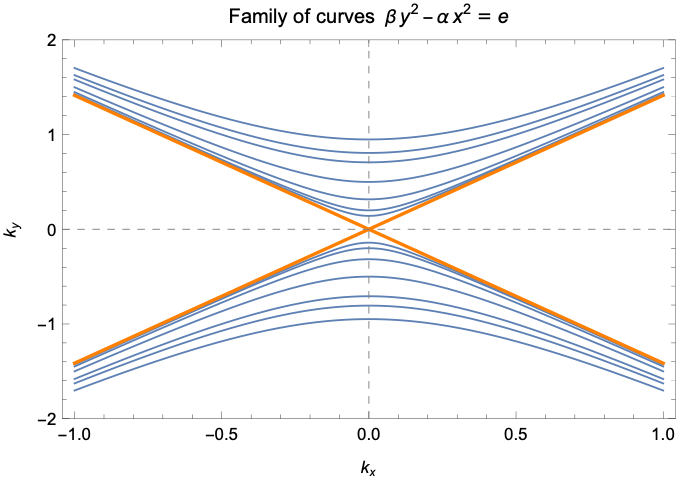
\includegraphics[width=\textwidth]{figures/introduction/logcontours.png}
        \caption{\centering conventional van Hove singularity, Eq.~\eqref{eq:dispQUAD}}
        \label{fig:logcontours}
    \end{subfigure}
    \hfill
    \begin{subfigure}[t]{0.45\linewidth}
        \centering
        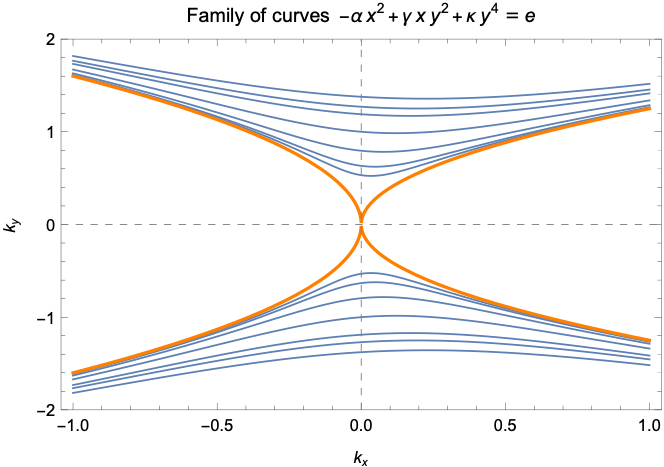
\includegraphics[width=\textwidth]{figures/introduction/paracontours.png}
        \caption{\centering higher order van hove singularity}
        \label{fig:paracontours}
    \end{subfigure}
    \hfill
    \caption{Hyperbolic geometry of the energy contours near a van Hove singularity. In each case, the limiting curve for $e=0$, which is here the van Hove energy, is shown by an orange line. More and more states can be fit into the corner created by the touching fermi surfaces at the van hove energy, leading to the diverging density of states.}
    \label{fig:vanHoveillustration}
\end{figure}

\par 
Near a conventional logarithmic van hove singularity, the contours of equal energy form hyperbolae in momentum space. This is easily visible in the topology change of the fermi surface, as it crosses the van hove energy. At exactly the van hove energy, the fermi surface is made of the asymptotes of the hyperbola, which are two lines meeting at a point. This can be generalized in many ways, the most obvious of which is to have a fermi surface composed of the intersection of two parabolae (see Fig. ~\ref{fig:paracontours}). This also has a direct effect in the type of singularity in the density of states: in this case being a power law~\cite{Yuan2019,Yuan2020PRB-classification}. These can be neatly classified by a recently developed catastrophe theory formalism~\cite{chandrasekaran2020catastrophe,classen2024high}
.  
\par
The higher order van hove singularity is believed to exist in many physical scenarios, most notably in the cuprates~\cite{markiewicz1989correlation,markiewicz2023investigating,paul2023exceptional} and in twisted bilayer graphene and other transition metal dichalcogenide bilayers.  

\section{Enhanced interactions near van hove points - towards Twisted Bilayer graphene}
Graphene is known to not be superconducting at charge neutrality owing to it being a bad metal~\cite{efetov2014towards}, i.e having a low density of states at the Dirac point. This can be understood in the following cartoon like picture. Assuming, BCS theory of superconductivity holds, the superconducting transition temperature is obtained by solving the linearized gap equation to be 
\begin{equation}
    T_c = \omega_0 \exp{-\frac{1}{g\rho(E_F)}},
    \label{eq:BCSTc}
\end{equation}
where $g$ is a parameter characterizing electron-electron attraction, $\omega_0$ is a UV cutoff (usually taken to be the Debye frequency) and $\rho(E_F)$ is the density of states at the fermi energy. The vanishing density of states of the Dirac cone implies an negative infinity in the exponential in Eq.~\eqref{eq:BCSTc}, meaning no superconductivity at any finite temperature.

\par
Thus it came as a surprise when twisted bilayer graphene was observed to be superconducting in some recent landmark experiments~\cite{Cao2018,Caocorrelated2018,oh2021evidence,lisi2021observation}. This is a part of a general phenomenon in which interactions get enhanced by the hyperbolic geometry in the fermi surface, which is sketched below. 










\section{The Kondo effect}



\section{This thesis}
In the introduction, we have explored different electronic systems, and identified clandestine hyperbolic geometries in each of them.  

\subsection{Chapter 1 - The Kondo effect in Twisted bilayer graphene}


\subsection{Chapter 2 - Chaos in the bipartite Sachdev-Ye-Kitaev model}



\subsection{Chapter 3 - Wormholes in the Yukawa-Sachdev-Ye-Kitaev model}

